\documentclass{handout}

% \SetInstructor{Lt Col James Phillips}
\SetCourseTitle{ECE231: Electrical Circuits and Systems I}
\SetSemester{Fall 2016}
\SetHandoutTitle{Lecture 36: Filters IV -- Filter Design Problems}

%\SetDueDate{1 Jan 2016}
%\ShowAllBlanks

\showsoln \setsolncolor{red}

\begin{document}
\maketitle

\textbf{OBJECTIVES:}
\begin{enumerate}
\item Demonstrate understanding by working filter design examples
\end{enumerate}

\textbf{READING}
\begin{description}
\item [Required]:
Filters Handout (Available on Sharepoint), pgs 39--45
\end{description}

This lesson is dedicated to doing example problems (board work).  Recommend you work on the board as I move around and help, but please copy the solution in your notes so you have access later.

\section{Example 1 -- Low Pass Filter}
\textbf{Given:}  We require a low-pass filter with a cut-off frequency of 2000 rad/sec and a passband gain of 20 dB.  Additionally, the filter must connect to a source with a Thevenin resistance of $5 \ k\Omega$.

\noindent \textbf{Find:}  Design a circuit that meets the specifications.

\soln{3in}{
\begin{figure} [h!]
\centering
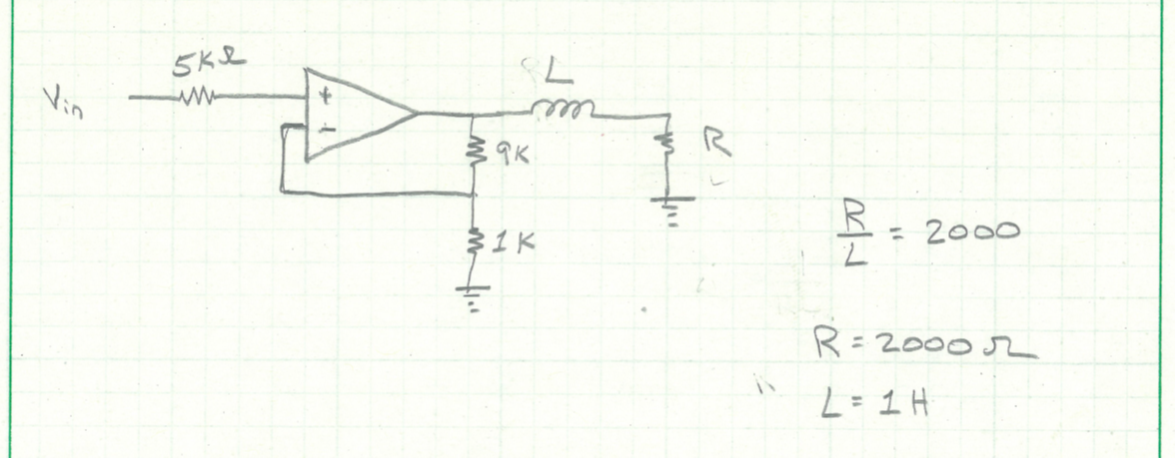
\includegraphics[width=1\textwidth]{Example1a.png}
\end{figure}

}

\soln{3in}{
\begin{figure} [h!]
\centering
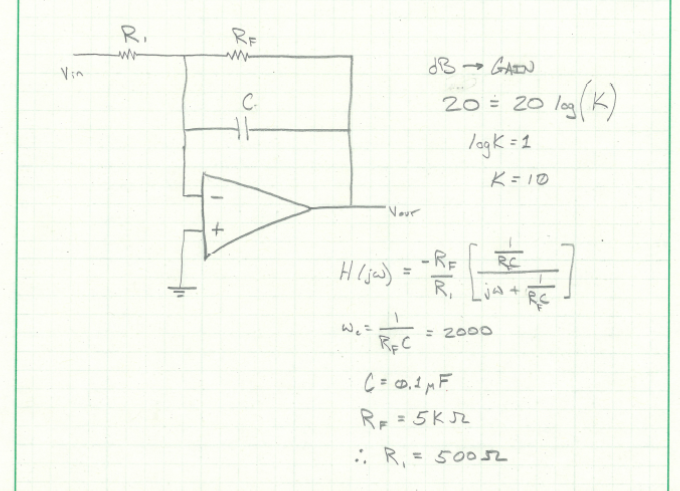
\includegraphics[width=1\textwidth]{Example1b.png}
\end{figure}

}
\newpage
\clearpage
\pagebreak

\section{Example 2 -- High Pass Filter}

\noindent \textbf{Given:}  We require a high-pass filter with a cut-off frequency of 318.31 Hz and a passband gain of $\pm$15.  Additionally, the filter must connect to a load with a resistance of $10 \ k\Omega$.

\noindent \textbf{Find:}  Design a circuit that meets the specifications.

\soln{6in}{
\begin{figure} [h!]
\centering
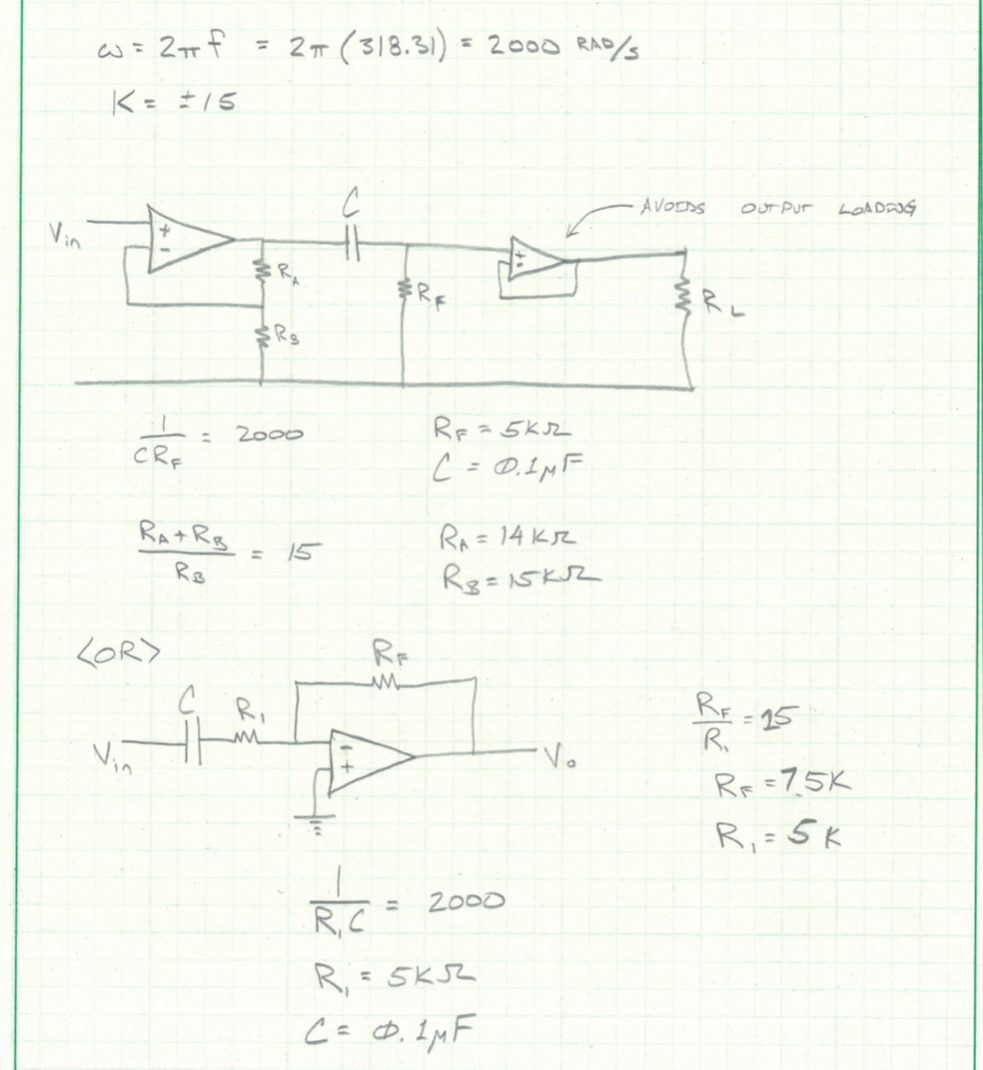
\includegraphics[width=1\textwidth]{Example2.png}
\end{figure}

}

\newpage
\clearpage
\pagebreak

\section{Example 3 -- Band Pass Filter}
\noindent \textbf{Given:}  We require a band-pass filter with a low cut-off frequency of 800 rad/sec, a high cut-off frequency of 20000 rad/sec,  and a passband gain of 40 dB.  Additionally, the filter must connect to a source with a Th\'{e}venin resistance of $10 \ k\Omega$ and a load with a resistance of $20 \ k\Omega$.

\noindent \textbf{Find:}  Design a circuit that meets the requirements.

\soln{6in}{
\begin{figure} [h!]
\centering
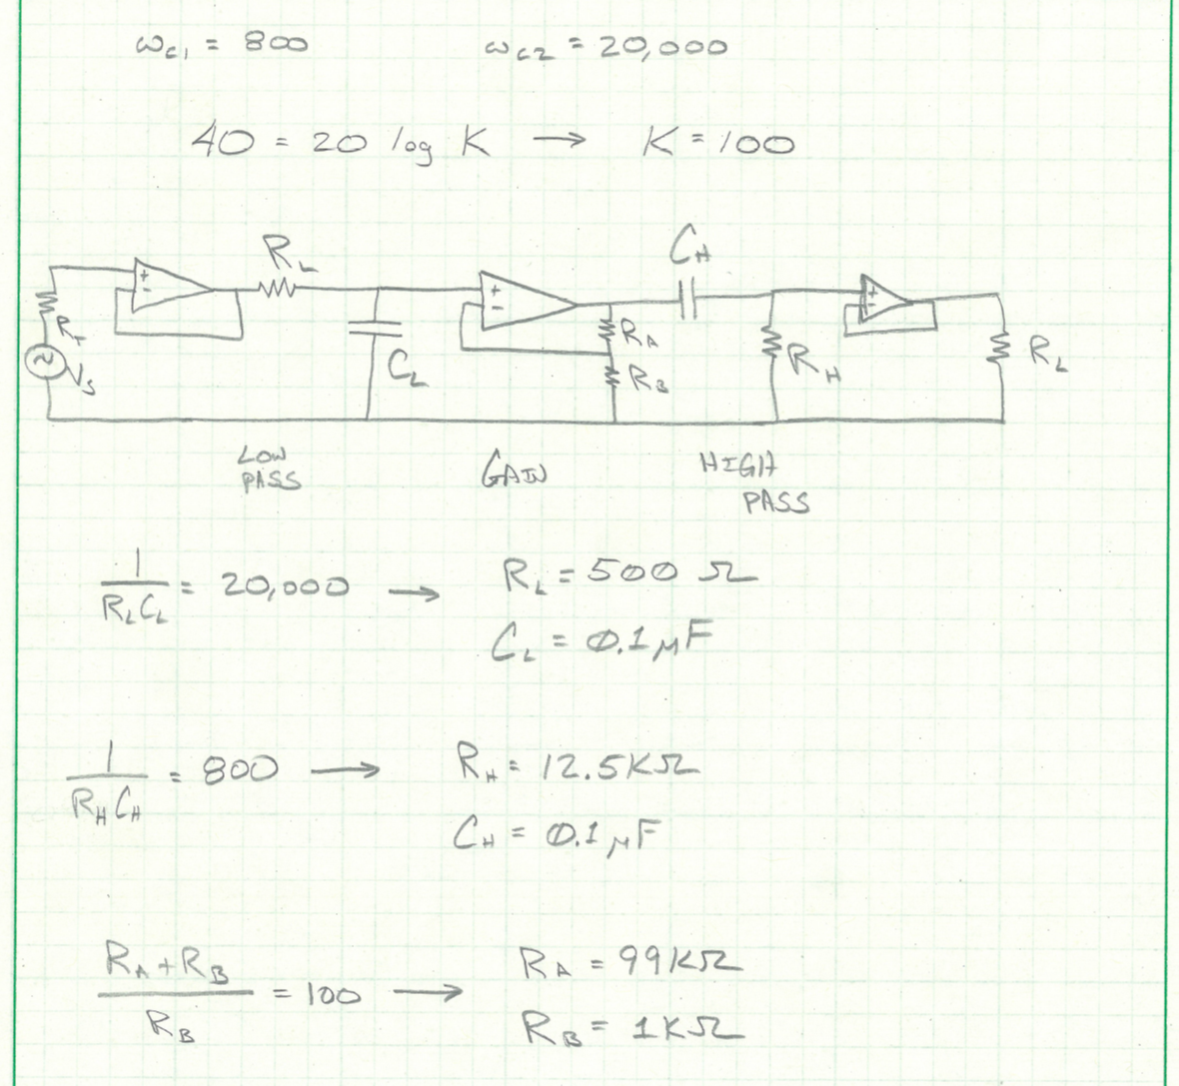
\includegraphics[width=1\textwidth]{Example3.png}
\end{figure}

}

\newpage
\clearpage
\pagebreak

\section{Example 4 -- Band Reject Filter}

\noindent \textbf{Given:}  We require a band-reject filter with a low cut-off frequency of 800 rad/sec, a high cut-off frequency of 20000 rad/sec,  and a passband gain of $\pm$100.

\noindent \textbf{Find:}  Design a circuit that meets the requirements.

\soln{6in}{
\begin{figure} [h!]
\centering
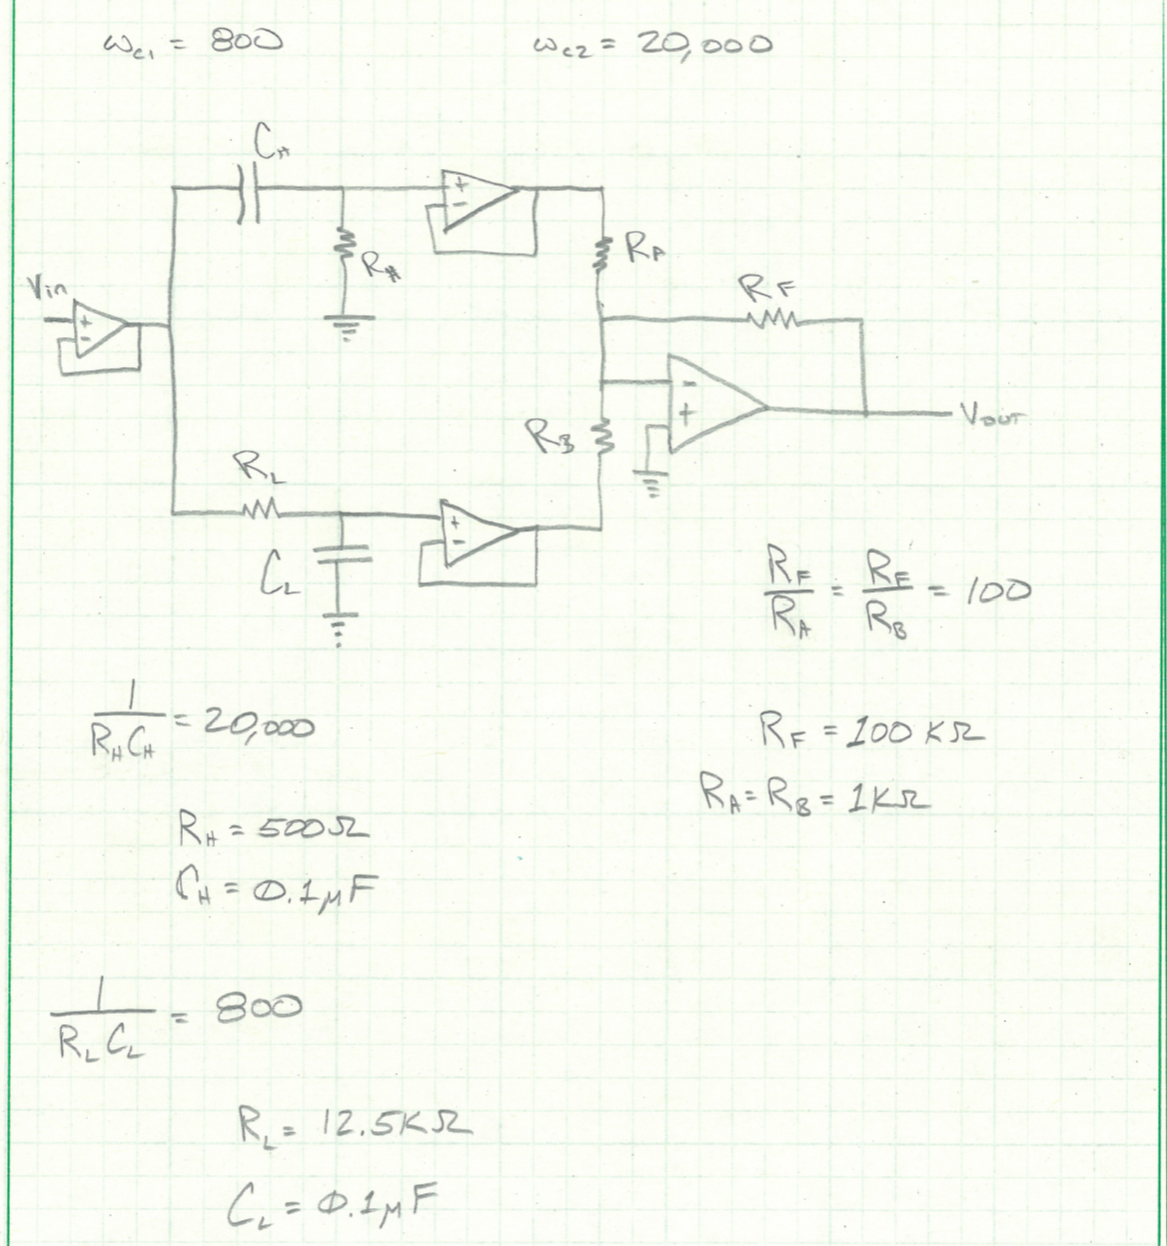
\includegraphics[width=1\textwidth]{Example4.png}
\end{figure}

}

\newpage
\clearpage
\pagebreak

\end{document}


% Equation Array Example Code
%\begin
%{eqnarray}
%P_R &=& i_R^2R \nonumber \\
%P_R &=& (100\ mA)^2 \times 100\ \Omega \nonumber \\
%P_R &=& (100 \times 10^{-3}\ A)^2 \times 100\ \Omega \\
%P_R &=& 10000 \times 10^{-6}\ A^2  \times 100\ \Omega \nonumber \\
%P_R &=& 1\ W  \nonumber
%\end{eqnarray}

% Figure Example Code
%\begin{figure} [h!]
%\centering
%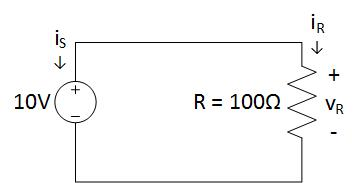
\includegraphics[width=0.5\textwidth]{OhmsLawExampleSolution.jpg}
%\caption{Ohm's Law example circuit}
%\label{fig: OhmsLawExampleSolution}
%\end{figure}

%Table Example Code
%\begin{table}[h]
%\centering
%\begin{tabular}{|l|c|c|}
%\hline
%Prefix & Abbreviation & Value \\
%\hline \hline
%Giga & $G$ & $10^9$ \\
%Mega & $M$ & $10^6$ \\
%Kilo & $k$ & $10^3$ \\
%\hline
%milli & $m$ & $10^{-3}$ \\
%micro & $\mu$ & $10^{-6}$ \\
%nano & $n$ & $10^{-9}$ \\
%pico & $p$ & $10^{-12}$ \\
%\hline
%\end{tabular}
%\caption{Engineering prefixes and values}
%\label{tab: Eng Prefixes}
%\end{table}
